\documentclass[svgnames,hyperref, english, xcolor=dvipsnames,usenames]{beamer}					      % version standard
%\documentclass[svgnames,hyperref, english, xcolor=dvipsnames,usenames,handout]{beamer}       		  % version imprimable pour assistance%
%\documentclass[svgnames,hyperref, english, xcolor=dvipsnames,usenames,handout,notes=show]{beamer}    % version imprimable avec notes d’orateur
%\documentclass[svgnames,hyperref, english, xcolor=dvipsnames,usenames,notes=only]{beamer}    		  % version imprimable avec notes d’orateur
\mode<presentation>
{
        \usepackage{beamerthemesplit}
        \usetheme[compress,secheader]{Madrid}
        \setbeamercovered{transparent}
}
\usepackage{amsthm}
\usepackage{amsfonts}
\usepackage{amsmath}
\usepackage{graphicx}
\usepackage{xspace}
\usepackage{stmaryrd}
\usepackage[utf8]{inputenc}
\usepackage[T1]{fontenc}
\usepackage[english]{babel}


%-----------------------------------------------------------

\definecolor{newcolor}{rgb}{0, 0, .90}
\definecolor{impcolor}{rgb}{.90, 0, 0}
\definecolor{darkergreen}{rgb}{0,0.5,0}
\definecolor{myorange}{rgb}{0.8,0.7,0}
\definecolor{myviolet}{rgb}{0.7,0.0,0.7}

\definecolor{lightpurple}{rgb}{0.83,0.27,1}
\definecolor{lightblue}{rgb}{0.27,0.9,0.9}


%\newcommand{\texthl}[1]{{\color{blue}#1}}
%\newcommand{\jaune}[1]{{\color{blue}#1}}
%\newcommand{\texthlb}[1]{{\color{orange}#1}}
%\newcommand{\orange}[1]{{\color{orange}#1}}
%\newcommand{\verte}[1]{{\color{green}#1}}
%\newcommand{\trad}{{\color{orange}{\bf $\leadsto$}}}

%\newcommand{\textcite}[1]{{\color{lightpurple}[#1]}}
%\newcommand{\textciten}[1]{{\color{lightpurple}#1}}

\newcommand{\texthl}[1]{{\color{red}#1}}
\newcommand{\jaune}[1]{{\color{red}#1}}
\newcommand{\texthlb}[1]{{\color{orange}#1}}
\newcommand{\orange}[1]{{\color{orange}#1}}
\newcommand{\verte}[1]{{\color{green}#1}}
\newcommand{\trad}{{\color{orange}{\bf $\leadsto$}}}

\newcommand{\textcite}[1]{{\color{myviolet}[#1]}}
\newcommand{\textciten}[1]{{\color{myviolet}#1}}

\newcommand{\montilde}{$\sim$}

\title[MarkUs]%
{MarkUs, a web based application to annotate student's code}

%\subtitle{}

\author[B. \textsc{Vialle}, G. \textsc{Guiot}]%
{Benjamin \textsc{Vialle}, Ghislain Guiot}
\institute[ECN]{\structure{École Centrale de Nantes}}

\date[2013-07-10]{LSM - 2013/07/10}

%\date[] % (optional)
%{}

\subject{Libre Software Meeting - 2013/07/10}

\AtBeginSection[] % Do nothing for \section*
{
        \frame<beamer>
        {
                \frametitle{Summary}
                \tableofcontents[current]
        }
}

\begin{document}

\frame{\titlepage}


\section{Introduction}

\frame
{
        \frametitle{Identified needs}

        \begin{alertblock}{Motivation}
                How to manage and evaluate the work performed by students in projects or in practical work?
        \end{alertblock}

        \begin{block}{Use}
                \begin{itemize}
                        \item Deployed at the École Centrale de Nantes since september 2010
                        \item Centrale Nantes is contributing to the development of MarkUs since summer 2009
                        \item MarkUs is used in
                                \begin{itemize}
                                        \item Teaching computer science (reports and source code)
                                        \item Class of more than 350 students
                                        \item More than 20 teachers impacted
                                \end{itemize}
                \end{itemize}
        \end{block}
}


\section{Context}

\subsection*{Motivation}

\frame
{
        \frametitle{Limitations of classic way to handle practical work}

        \begin{alertblock}{Teachers side}
                \begin{itemize}
                        \item Important \textbf{number} of submissions to handle (hundreds by practical work)
                        \item Difficulty of harmonizing correction factors between graders
                        \item Paper handling
                                \begin{itemize}
                                        \item Accumulation of papers containing source code
                                        \item Giving back papers to students
                                \end{itemize}
                        \item Email handling
                                \begin{itemize}
                                        \item Mistakes in the grader's name
                                        \item Zip archives not readable
                                        \item Not a smooth process
                                \end{itemize}
                \end{itemize}
        \end{alertblock}
}

\frame
{
        \frametitle{Limitations of classic way to handle practical work}

        \begin{alertblock}{Students side}
                \begin{itemize}
                        \item Difficulty to have \textbf{feedback} on his work
                        \item Paper handling
                                \begin{itemize}
                                        \item Loss of reports
                                        \item How to \textbf{share} correction with his co-worker?
                                \end{itemize}
                        \item Email handling
                                \begin{itemize}
                                        \item Mistakes in student's names
                                        \item An email among others
                                \end{itemize}
                \end{itemize}
        \end{alertblock}
}

\subsection*{MarkUs}

% Quelques mots de présentation historique autour de MarkUs

\frame{
        \frametitle{MarkUs, an online marking tool}
        \begin{block}{MarkUs? Mark us!}
                MarkUs is:
                \begin{itemize}
                        \item a \textbf{web} application
                        \item Aimed at \textbf{grading assignments} in computer science
                        \item \textbf{Versioned} repository of student's work
                        \item \textbf{Direct annotation} of documents by teachers
                        \item Reduced \textbf{time} of correction
                \end{itemize}
        \end{block}
}

\frame{
        \frametitle{Organization around MarkUs}
        
        \begin{block}{MarkUs team}
                Karen Reid, senior lecturer at the University of Toronto, team leader\\
                Morgan Magnin, associate professor at the École Centrale de Nantes, managing french student projects
                \begin{itemize}
                        \item 4 core developers
                        \item  Quarterly team of students
                        		(Canadian and French)
                        \item Several Universities are using MarkUs
                        	  	(Canadian and French)
                        \item Collaborative development on Github
                \end{itemize}
        \end{block}
}

\frame{
        \frametitle{Some features}

        \begin{block}{Improving teaching (grader)}
                Possibility to \textbf{annotate}
                \begin{itemize}
                        \item Source code (with syntax highlighting)
                        \item Images
                        \item PDF
                \end{itemize}
                \vspace{-1em}
                \begin{figure}
                        \begin{center}
                                \scalebox{0.61}{
                                        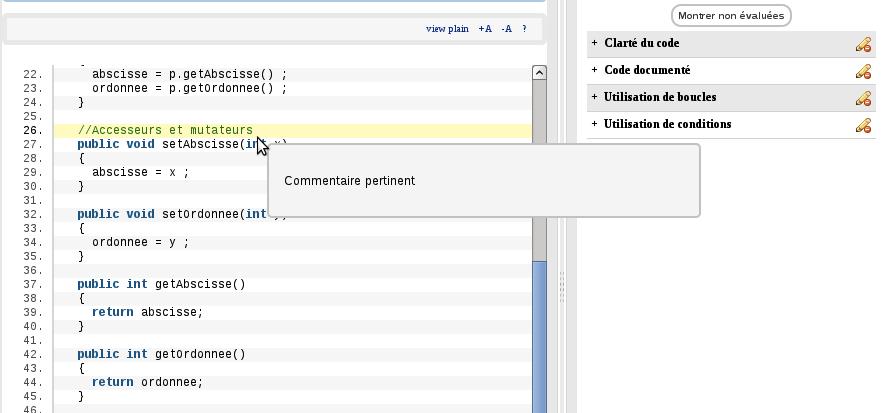
\includegraphics[width=\textwidth]{images/markus-annotations.png}
                                }
                                %
                                \caption{Grader view}
                        \end{center}
                \end{figure}
        \end{block}
}

\frame{
        \frametitle{Some features}

        \begin{block}{Improving teaching (grader)}
                \begin{itemize}
                        \item \textbf{Fixed} assessment criteria
                        \item Annotations (source code, images and PDF)
                        \item More than one grader on a paper
                        \item Grader management by criteria
                \end{itemize}
                \vspace{-1em}
                \begin{figure}
                        \begin{center}
                                \scalebox{0.29}{
                                        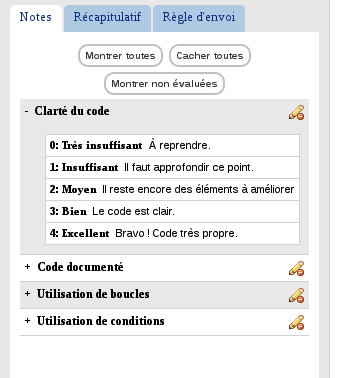
\includegraphics[width=\textwidth]{images/markus-criteres.png}
                                }
                                %
                                \caption{Set of criteria}
                        \end{center}
                \end{figure}
        \end{block}
}

\frame{
        \frametitle{Some features}

        \begin{block}{Improving teaching (grader)}
                \begin{itemize}
                        \item Handling many practical work, with one instance of MarkUs per course
                        \item Managing \textbf{deadlines} with configurable penalties
                        \item Possibility to see and grade a \textbf{former} version
                \end{itemize}
        \end{block}
}

\frame{
        \frametitle{Some features}

        \begin{block}{Improving teaching (student)}
                \begin{itemize}
                        \item Creating groups \textbf{for each practical work}
                        \item \textbf{Exporting} annotations
                        \item Better and faster feedback
                        \item Possibility to read annotations until the evaluation
                		%%%%%%%
                		% TODO: faire un point sur les remark requets
                		%%%%%%%                        
                        \item Can create \textbf{remark request}
                \end{itemize}
                \vspace{-1em}
                \begin{figure}
                        \begin{center}
                                \scalebox{0.55}{
                                        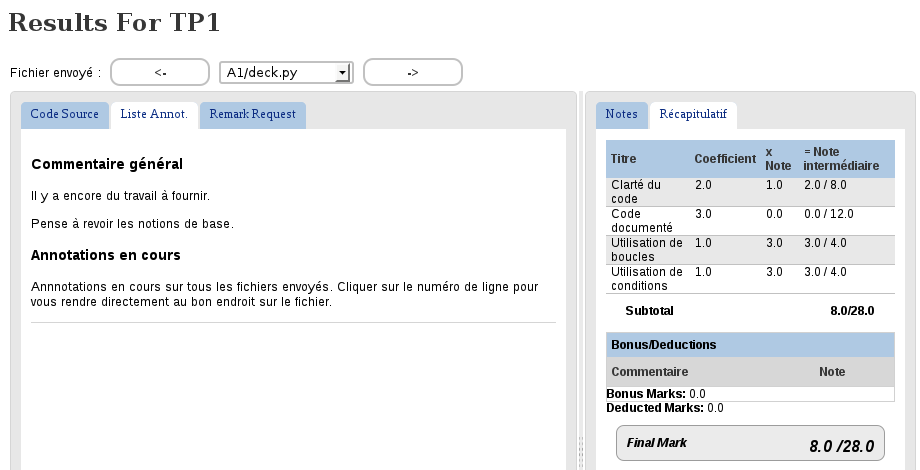
\includegraphics[width=\textwidth]{images/markus-commentaires.png}
                                }
                                \caption{Result view for students}
                        \end{center}
                \end{figure}
        \end{block}
}

\frame{
        \frametitle{Some features}

        \begin{exampleblock}{\emph{Release} of MarkUs 1.0}
                \begin{itemize}
                	\item Compatibility Ruby 1.9.3 and Ruby on Rails 3.x
                	\item \textbf{Sections} inside of a class
                	\item Conversion of PDF \textbf{instantaneous}
                	%%%%%%%
                	% TODO: faire un point sur les remark requets
                	%%%%%%%
                	\item Added \textbf{remark requests}
                	\item \textbf{New dashboard} for admin
                \end{itemize}
%                \vspace{-1em}
%                \begin{figure}
%                        \begin{center}
%                                \scalebox{0.55}{
%                                        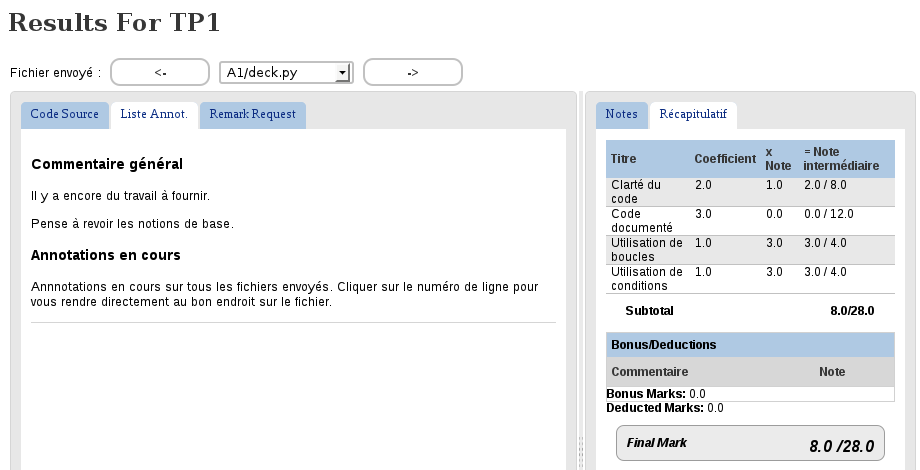
\includegraphics[width=\textwidth]{images/markus-commentaires.png}
%                                }
%                                \caption{Vue des résultats par les étudiants}
%                        \end{center}
%                \end{figure}
        \end{exampleblock}
}

\subsection*{Demonstration}

\frame{
        \frametitle{Demo}
        And what about seeing MarkUs in action?
}



\section{Impact on teaching and learning}

% Cette partie pour donner un aperçu des fonctionnalités de MarkUs et leur impact sur l'enseignement

\subsection*{Benefits for teachers}

\frame{
        \frametitle{Why MarkUs seduces teachers?}
        \begin{itemize}
                \item Managing \textbf{large volumes}
                \item \textbf{Centralized} document management
                \item \textbf{Reduced time} for grading (around 50\%)
                \item \textbf{Paperless}
                \item \textbf{Mobile} access
        \end{itemize}
}

\subsection*{Benefits for students}

\frame{
        \frametitle{Why MarkUs seduces students?}
        \begin{itemize}
                \item \textbf{Unique} platform to submit and get feedback for practical work
                \item \textbf{Permanent} access to former work graded by teachers
                \item Improved \textbf{time} for obtaining the correction
        \end{itemize}
}

\subsection*{Use at Centrale Nantes}

\frame{
        \frametitle{At Centrale Nantes}
        
        \begin{block}{Deployment of MarkUs for computer science courses}
                \begin{itemize}
                        \item Since September 2010
                        \item Connected to \textbf{LDAP}
                        \item Used in first and second year:
                                \begin{itemize}
                                        \item 370 and 340 students
                                        \item 21 teachers
                                \end{itemize}
                        \item \textbf{Computer science} class:
                                \begin{itemize}
                                        \item Algorithm
                                        \item C
                                        \item Java
                                \end{itemize}
                \end{itemize}
        \end{block}
}

\frame{
        \frametitle{Advantages of MarkUs}
        \begin{block}{Student side:}
                \begin{itemize}
                        \item Pedagogical effect of \textbf{reaching deadlines}
                        \item \textbf{Individual access} to the graded work of his group
                        \item \textbf{More consultation} of the annotations left by teachers
                \end{itemize}
        \end{block}
}

\frame{
        \frametitle{Advantages of MarkUs}
        \begin{block}{Teacher side:}
                \begin{itemize}
                        \item Improved \textbf{logistics} management
                        \item An initial \textbf{standardization} of criteria
                        \item \textbf{Incentive} effect for the correction
                \end{itemize}
        \end{block}
}

\section{MarkUs deployment}

\frame{
        \frametitle{Around MarkUs}
        \begin{block}{Practical modalities}
                \begin{itemize}
                        \item Written in Ruby, with Ruby on Rails
                        \item Documents saved with subversion
                        \item Access through a web interface
                        \item Expert users: access using CLI and REST API
                \end{itemize}
        \end{block}
        
        \begin{block}{Try it!}
                \begin{itemize}
                        \item Virtual machine: already configured MarkUs instance
                \end{itemize}
        \end{block}
}


\section{Conclusion}


\subsection*{Bilan}

\frame
{
        \frametitle{Synthèse}

        \begin{alertblock}{MarkUs, an online marking tool to annotate student's code}
                How to improve evaluation process in practical work or student's projects?
        \end{alertblock}

        \begin{block}{MarkUs}
                \begin{itemize}
                        \item Free software
                        \item Annotation of \textbf{source code}, \textbf{images} and \textbf{PDF}
                        \item Easy to use
                        \item Only cost: installation and maintenance
                        \item Usage popular with students and teachers
%                        \item Vers la création de \textbf{cercles vertueux} : utilisateurs $\rightarrow$ contributeurs $\rightarrow$ mentors
                \end{itemize}
        \end{block}
}

\subsection*{Perspectives}

\frame{
        \frametitle{Next features}

        \begin{block}{Extend the use of MarkUs}
                \begin{itemize}
%                        \item Analyse plus fine des effets du dispositif pédagogique
                        \item \textbf{Tactile annotation} module
                        \item Integration of \textbf{mathematical annotations}
                        \item \textbf{Automated testing} of student's code
                        \item Extend MarkUs to other courses
                        \item Integration to a \textbf{VLE}\footnote{Virtual Learning Environment} ?
                        \item Easy deployment using virtual machines
                \end{itemize}
        \end{block}
}

\subsection*{References}

\frame{
        \frametitle{More information}

        \begin{block}{Links and contacts}
                \begin{itemize}
                        \item Project website: \url{http://markusproject.org}
                        \item Try it online: \url{http://demo.markusproject.org}
                        \item GitHub repository: \url{https://github.com/MarkUsProject/Markus}
                        \item Blog EAT-TICE of the École Centrale de Nantes: \url{http://eat-tice.ec-nantes.fr}[FR]
                        \item IRC channel: \#markus sur irc.freenode.net
                        \item Mailing list: \url{markus-dev@markusproject.org}
                \end{itemize}
        \end{block}
}

%\bibliography{biblio}
%\bibliographystyle{alpha}

\end{document}
